\section{Robust classification}
\label{sec:robustness}

%\begin{figure*}[!t]
%\vskip 0.2in
%\begin{center}
%\begin{subfigure}[b]{0.4\textwidth}
 % 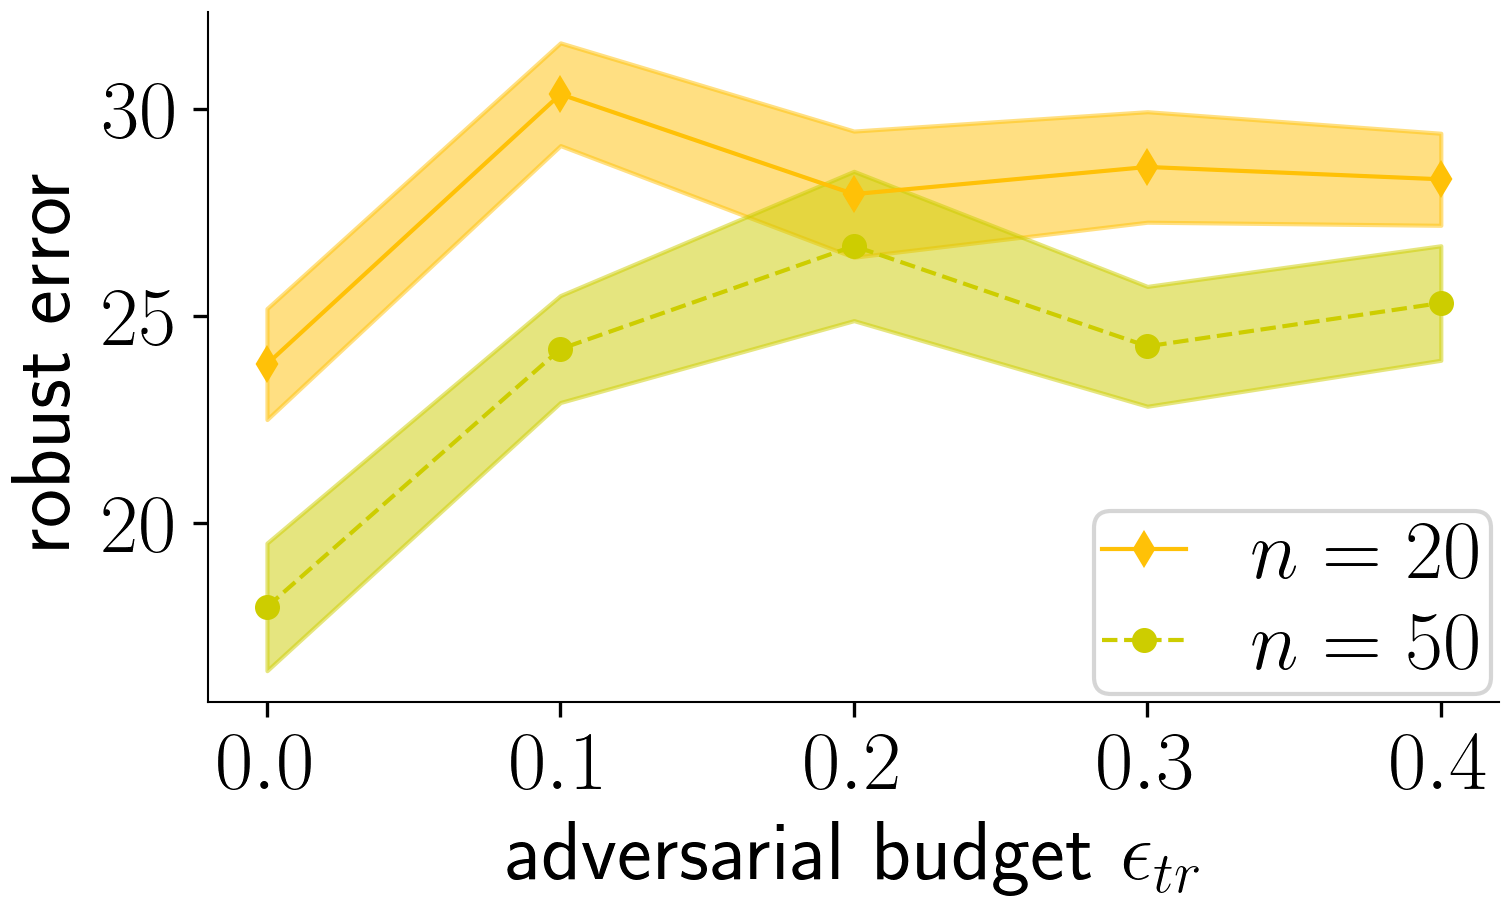
\includegraphics[width=0.99\linewidth]{plotsAistats/water_birds_light_d_n.png}
 % \caption{Waterbirds illumantion attack}
  %\label{fig:eps_cs}
%\end{subfigure}
%\caption{We plot the robust accuracy as a function of the adversarial budget $\epstrain$ used during training for (a) logistic regression on a sparse ground truth with $d=1000,\epstest=4$ with varying sample size  and (b) a ResNet50 fit on the waterbirds data with increasing adversarial lighting. Note that for all experiments, if $d/n$ is small enough, then adversarial training increases the resulting robust error. Experimental details can be found in Sections~\ref{sec:logregapp} and \ref{sec:app_waterbirds}}
%\label{fig:eps_panel}
%\end{center}
%\end{figure*}


We first introduce our robust classification setting more formally by defining
the notions of  adversarial robustness, \nameofattacks and adversarial training
used throughout the paper.


\paragraph{Adversarially robust classifiers}

For inputs $x \in \R^\dims$, we consider multi-class classifiers
associated with parameterized functions $f_\theta:\R^\dims \to
\R^\numlabels$, where $\numlabels$ is the number of labels. In the special case of binary classification ($\numlabels = 2$), we use the output predictions $y=\textrm{sign}(f_\theta(x))$. For example, $f_\theta(x)$ could be linear models (as in Section~\ref{sec:theoryresults}) or
neural networks (as in Section~\ref{sec:realworldexpapp}).
%and provide experimental evidence of our phenomenon \fy{here 'd be nice to have name} with neural networks $f_\theta$.

%One key step to convince data-scientists and engineers to employ machine learning based classification for real-world applications,  is to increase their
One key step to encourage deployment of machine learning based classification in real-world applications, is to increase the
robustness of classifiers against perturbations that do not
change the ground truth label. 
% is one of the key requirements that need to be fulfilled. 
%% For instance, in image classification, adding a small sticker to an image or rotating an image should not alter its prediction, provided the human
%% classification stays the same.
Mathematically speaking, we would like to have a small
\emph{$\epstest$-robust error}, defined as
\begin{equation}
  \label{eq:roberr}
  \roberr{\theta} := \EE_{(x, y)\sim \prob} \max_{x' \in \pertset{x}{\epstest}} \ell(f_\theta (x'),y),
\end{equation}
where $\ell$ is the multi-class zero-one loss, which only equals $1$ if the predicted
output using $f_\theta(x)$ does not match the true label $y$.
Further, $\pertset{x}{\epstest}$ is a perturbation set associated with a \emph{transformation type} and size $\epstest$. 
Note that the \emph{(standard) error} of a classifier corresponds to evaluating $\roberr{\theta}$ at $\epstest = 0$, yielding the standard error $\stderr{\theta} =\EE_{(x, y)\sim \prob} \ell(f_\theta (x),y)$.

\paragraph{(Signal)-Directed attacks}
Most works in the existing literature consider consistent perturbations where
$\epstest$ is small enough such that all samples in the perturbation set
have the same ground truth or expert label. 
Note that the ground truth model $f_{\theta^{\star}}$ is therefore robust against perturbations and achieves the same error for standard and adversarial evaluation. 
%do not hinder the classification by an expert or the ground truth.
The inner maximization in Equation~\eqref{eq:roberr} is often called the adversarial \emph{attack} of the model $f_\theta$ and the corresponding solution is referred to as the adversarial example.
In this paper, we consider \emph{\nameofattacks}, as described in Section~\ref{sec:intro}, that effectively reduce the information about the ground truth classes.
Formally, we characterize \emph{\nameofattacks} by the following property: 
for any model $f_\theta$ with low standard error, the corresponding adversarial example is well-aligned with the adversarial example found using the ground truth model 
$f_{\theta^{\star}}$.
%adversarial examples computed with respect to  models $f_\theta$ with low standard error
%are well-aligned with the adversarial example found using %the ground truth model 
%$f_{\theta^{\star}}$.
An example for such an attack are additive perturbations that are constrained to the direction of the ground truth decision boundary.  We provide concrete examples for linear classification in  Section~\ref{logreg_linear_model}.
 

%The evaluation metric
%$\ell$ is the multi-class zero-one loss, which only equals $1$ if the predicted
%output using $f_\theta(x)$ does not match the true label $y$.

%For simplicity, we often refer to the errors of a classifier associated with $\theta$ as the error of $\theta$.

%% In \emph{adversarially robust} classification, we would like the
%% prediction to be invariant or robust against attacks. 
%%  More generally, we have an \emph{attack-model}
%% in mind, that we want to be robust against.

%% More precisely, 
%% an attack model $\attackmodeltest$ takes as input a data point $(x,y)$ and outputs an
%% adversarial example $\tilde{x}$ that depends on a \emph{perturbation set} $\pertset{x}{\epstest}$ of $x$ with
%% \emph{perturbation set size} $\epstest$, and an algorithm $\algo$, i.e.
%% \fy{loss we just assume is always the zero one?}
%% \begin{equation}
%%   \label{eq:attackmodel}
%%   x' = \attackmodeltest(x, y; \pertset{x}{\epstest}, \algo(\theta)).
%% \end{equation}
%% where the $\algo$ tries to find an example in $\pertset{x}{\epstest}$ that is ``bad''.

%% Furthermore, we define the \emph{$\epstest$-robust
%%   accuracy} of a classifier induced by parameters $\theta$ as 
%% \begin{equation}
%%   \label{eq:robacc}
%%   \robacc{\theta} := \EE_{(x, y)\sim \prob} \Indi{y f_\theta (\attackmodeltest(x,y; \pertset{x}{\epstest}, \algo)) >0}
%% \end{equation}
%% where $\Indi{E}$ is the indicator function and equals to one if the
%% event $E$ is satisfied and zero else.\footnote{Note that the
%%   \emph{(standard) accuracy} of a classifier can be calculated from an
%%   expression for $\robacc{\theta}$ by evaluating it at $\epstest = 0$,
%%   yielding $\stdacc{\theta} = \EE_{x,y\sim \prob} \Indi{y f_\theta (x)
%%     >0}$}
%% For simplicity, we often refer to the different
%% accuracy of a classifier associated with $\theta$ as the accuracy of
%% $\theta$.

%% \fy{write sth meaningful} Our theoretical results uses the common
%% definition of adversarial robustness that assumes perfect adversarial
%% examples where the algorithm finds the minimum in a perturbation set
%% that is
%% \begin{equation}
%%   \label{eq:exactattack}
%%   \attackmodeltest(x, y; \pertset{x}{\epstest},\algo(\theta)) =
%%   \min_{x' \in \pertset{x}{\epstest}} \Indi{y f_\theta (x') >0}
%% \end{equation}
%% so that we have
%% \begin{equation}
%%   \label{eq:minrobustness}
%% \robness{\theta} : = \EE_{x\sim \prob} \min_{x' \in
%%   \pertset{x}{\epstest}} \Indi{y f_\theta(x') >0}.
%% \end{equation}
%% However, in practice exact search is rarely possible unless the set is
%% discrete (certificates go overboard) and the algorithm matters. In our
%% examples we study both exact search (mask attacks) as well as effect
%% of algorithm strength ($K$ for masks, grid resolution for blur etc.)


%%\paragraph{(Signal)-Directed attacks}

%%The transformations we consider in this paper are 
%%\fy{this is bullet point style}
%%In Section~\ref{sec:intro} we introduced the concept of \nameofattacks
%%as ones that can efficiently use budget bla

%%For object recognition, these could be occlusion or corruption attacks specifically applied on the object, such as stickers or motion blur. More abstractly speaking, they should effectively transform core features that are used to recognize the object, such as texture, color, shape etc.

%%In the theoretical section, we formally model \nameofattacks
%%for additive perturbations as follows: 
%%Suppose that an attack returns
%%$ x+ \delta$ where $\delta$ depends on the model $\theta$.
%%Further assume
%%that the shortest path from some $x$ to the decision boundary is in the
%%direction $v$ (we say, the \emph{signal} direction).
%% types \fy{in some feature space?} and assume
%% that shortest path from some $x$ to the decision boundary is in the
%% direction $v$ (we say, the \emph{signal} direction).
%% Further, 
%% given a perturbation budget $\epstrain$, assume that an additive perturbation
%% \nameofattack returns some adversarial example $ x+ \delta$ where
%% $\delta$ depends on the model $\theta$.
%%We then call $T$ a \nameofattack if for most models $\theta$, $\delta$ directionally aligns with $v$.

%%Concretely for linear models for example, this would be linfty set. (not sure i'd mention l1 set here?)

%%owever for general $\ell_p$ perturbations this is not satisfied. 

%%Certinaly this notion can be extended to additive perturbation in arbitrary feature spaces - this then becomes closer to the image ones we discussed.

%%\jc{In Section~\ref{sec:intro}, we defined attacks that efficiently use their perturbation budget to decrease the information about the class in the input as directed attacks. In the setting of object recognition, these could be occlusions or transformations on the object such as the stickers and motion blur. More abstractly, directed attacks on images transform core features of the object, which are used to recognize the object. Examples of core features are texture, color and shape of the object.}

%% We now define \nameofattacks slightly more
%% generally.  In Figure \ref{fig:sig_att_examples}, we show three examples of
%% %physical, masks on boats? 
%% perceptible perturbations that make it harder to classify the object by decreasing the information about the class in the image.
%% All three transformations are perceptible and target some
%% of the core features, which are used to recognize the
%% object. In this paper, we refer to such attacks as \emph{\nameofattacks}.
%% Moreover, in this work, we consider consistent perturbations:
%% %the presented perturbations 
%% the attacks are small enough such that they do not hinder the classification by an expert or the ground truth. 
%% %\jc{In this paper, we refer to attacks that make classification harder by reducing the information about the class in the sample, while retaining the true class label, as consistent \emph{\nameofattacks}}.

%% %We call such attacks, that make classification harder by reducing the information about the class in the sample, \emph{\nameofattacks}. Moreover, in this paper, we focus on \nameofattacks that retain the true class label, i.e. \emph{consistent} \nameofattacks.

%% Undirected attacks may include directed perturbations, e.g. $\ell_p$-attacks for large enough $\epsilon$ contain motion blur perturbations. However, for directed attacks, the search space is constrained and biased
%% towards the direction of the optimal decision boundary. In contrast, $\ell_p$-attacks may even for large
%% $\epsilon$ attack in all directions and regions of the image.
%% This paper discusses the surprising phenomena that occur with
%% \nameofattacks and questions the applicability of common practices used for traditionally studied imperceptible undirected attacks.

%% We now motivate the type of perturbations that
%% we consider in this paper.  Consider the goal is to recognize objects.
%% However in the wild, the object might not appear the same way as in
%% the training data. These changes may or may not be intentional. \fy{but
%%   this doesn't play a role for us}

%% For example, animals could be moving at different speeds, causing
%% motion blur (which also depends on the camera settings that might
%% differ between photographers); they might adapt their color to their
%% environment or reduce contrast \fy{dunno if they do} to protect
%% themselves from predators. For animal detection, such natural
%% transformations might Recently, criminal face detection \fy{faced}
%% another unexpected challenge with masks of different sizes, covering
%% potentially key features of the face (nose, mouth), depending on how
%% they are worn. \fy{can get rid of one of these examples - lengthy?}
%% %with the mask mandates where key features of the face are now covered,
%% %sometimes worn in different locations 

%% %% Examples: masks on humans that can be of different size or location,
%% %% moving objects of different speed (motion blur), or animals that
%% %% adapt to their environment to fool predators.
 
%% An optimally robust model should ideally recognize the objects
%% irrespective of such transformations\fy{perturbations} since the objects
%% identity is unchanged (in other words consistent/content-preserving). If the
%% distribution of such changes were known or observed, one could
%% optimize the loss on that shifted distribution by using tools from
%% domain adaptation \fy{cite}.  Usually however, the distribution is
%% unknown in which case distribution shift or adversarial (worst-case)
%% robustness may be a good goal to aim for.




%% We refer to \emph{perturbation sets} $\pertset{x}{\epsilon}$ that
%% preserve the label, as \emph{consistent} perturbations of size
%% $\epsilon$ \fy{also called content-preserving by gilmer}. 
%% \fy{why consistent is relevant - might be obvious can cut- but good to keep in mind}
%% For traffic signs, the GT is the
%% human labeler, and the attacker might want to harm self-driving cars
%% only without getting reported to the police and hence defeats the purpose.
%% In the case of blurs you want to be good throughout a range of
%% optical and photographic qualities - for which you have no prior knowledge.

%% A lot of focus in the image classification robustness literature has
%% been devoted to $\ell_p$- perturbations \fy{maybe define?}.  If an
%% attacker has a budget $\epsilon$ \fy{for consistency} in terms of e.g. $\ell_p$ input
%% perturbation - they can attack the input in many directions.
%% For example if the model might use spurious correlations in a small
%% sample / imbalanced dataset like the background and the object itself. 

%% When the model is known (white-box), they could concentrate the attack
%% on directions that are most used by the model at hand (useful
%% non-robust features). When the model is not known (black-box) or only
%% known to give good predictions, we consider attacks that concentrate
%% on the most useful features for the \emph{ground truth} classifier.
%% These attacks are likely perceptible and motivated by fact the that
%% even the ``best'' models would crack under this (though funnily the
%% ones that learn spurious correlations would not, if its still
%% spuriously correlated). For image object classification for example,
%% such an attack might focus on the region wheer the major features of
%% the object are - such as stickers or watermarks on traffic signs
%% \cite{Eykholt18} and corruptions such as motion blur specifically on
%% the object, see Figure \ref{fig:sig_att_examples}).

%% One can also view this as a train-test shift.  In the
%% labeled data, you might not see stickers and similarly the training
%% images might be taken online with good photographs have short enough
%% exposure not to pick up the motion blur of a flying bird - as opposed
%% to the hobby bird photographer that uses worse optics.
%% Since the distribution of sticker size / locations or optical quality
%% are usually unknown a priori, ideally, for a robust system, you desire to perform well for
%% any such attacks up to a budget $\epsilon$ for which all perturbations
%% in the set $\pertset{x}{\epsilon}$ are still consistent - i.e. it
%% does not change the ground truth label.
%% \fy{if its truly blackbox, then you don't have to / can't do the search
%%   and just put $\epsilon$ done}

%% Theoretically speaking, we can model such attacks as constrained
%% $\ell_p$ attacks where the constraints direct the attack in the
%% direction that has the closest distance to the decision boundary. 

%% \fy{something I like but probably will cut} Animals also try to attack the
%% classification model of other animals by completely adapting their appearance
%% to the surroundings and hence significantly reducing the signal (the features
%% that one usually uses to detect them).

%% \fy{this one could perhaps be moved maybe to related work} In the
%% labeled data, you might not see stickers and similarly the training
%% images might be taken online with good photographs have short enough
%% exposure not to pick up the motion blur of a flying bird - as opposed
%% to the hobby bird photographer that uses worse optics.  Hence, this
%% can also be viewed as distribution shift problem.  Corruptions for
%% example, have been studied in this context.  There they consider a
%% distribution over attack-strength - forming a new distribution and
%% then want to perform well on that.  However since we do not know the
%% distribution in advance, in safety-critical matters, knowing the
%% space of attacks, worst-case (distribution shift robustness) makes
%% more sense.

%% \fy{maybe somewhere related work}
%% Instead of
%% worst-case, corruptions like motion blur for example have so far been
%% primarily used to study domain adaptation and average-corruption accuracy
%% \fy{cite}. We argue that the adversarial robustness perspective on
%% such kind of corruptions is relevant as well - after all in security one would like
%% to have good 



%% In this paper, we focus on perceptible consistent
%% perturbations that make it harder for a human to
%% distinguish objects from different classes.
%% Some realistic examples for natural images include for example
%% stickers on stop signs \cite{Eykholt18}, but also some common image corruptions such as motion blur (Figure \ref{fig:WB_motion_blur}), which arises when photographing fast moving objects.
%% All such perturbations are perceptible and effectively target the signal component in the data, but still do not change the label; they are in the classification of \cite{gilmer18b}, "content-preserving perturbations". In Figure \ref{fig:sig_att_examples}, we plot two examples of signal-attacking perturbations, which we use in experiments on real-world datasets. In the next section, we consider linear models and model such signal-attacking perturbations by considering transformations that move the input closer to the decision
%% boundary.


%% Note that corruptions are for example also studied in the context of distribution shifts or invariances. Classically, these works have as goal the accuracy on an unknown average distribution shift. Nevertheless, in multiple settings such as animals hiding through color-matching (by eg. a chameleon) or maliciously chosen perturbations and corruptions, robustness against the worst-case corruption is key. 

\paragraph{Adversarial training}

%%Typically, to minimize the robust test loss~\eqref{eq:roberr}, the ERM equivalent
%%defense mechanism would be to minimize the robust training objective
%% with a convex surrogate classification loss $\loss$ such as the cross-entropy loss.

%% Adversarial training often runs (stochastic) gradient descent on a proxy
%% classification loss using a particular attack-model. That is, defining $x' =
%% \attackmodeltest( \theta^{t-1})$ in each iteration we run
%% \begin{equation}
%%   \label{eq:sgdrob}
%%   \theta^t = \theta^{t-1} - \eta_t \nabla_\theta \ell (f_{\theta^{t-1}}(x_i')y_i)
%% \end{equation}
%% Common wisdom is that one should use the same attack model
%% In particular, robustness does not transfer between attack models (references)
%% However we focus on  ...

In order to obtain classifiers with a good robust accuracy, it is
common practice to minimize a (robust) training objective $\mathcal{L}_{\epstrain}$ with a surrogate
classification loss $\loss$ such as
\begin{equation}
  \label{eq:emploss}
  \robloss{\theta} :=  \frac{1}{n} \sum_{i=1}^n \max_{x_i' \in \pertset{x_i}{\epstrain}} \loss(f_\theta(x_i') y_i),
\end{equation}
which is called adversarial training.  In practice, we often use the
cross entropy loss $\loss(z) = \log (1+ \E^{-z})$ and minimize the
robust objective by using first order optimization methods such as
(stochastic) gradient descent.  SGD is also the algorithm that we
focus on in both the theoretical and experimental sections.


When the desired type of robustness is known in advance, it is
standard practice to use the same perturbation set for training as for
testing, i.e. $\pertset{x}{\epstrain}=\pertset{x}{\epstest}$. For example, \citet{madry18} shows that the robust error sharply increases for $\epstrain < \epstest$.
%\fy{catastrophic overfitting shows when attack is weaker its worse} 
%For example, in the case of \nameofattacks, one may insert motion blur or masks
%specifically on the object. 
%% sits for example - you could just insert corruptions such as masks or
%% train with motion blur on the object.
%%In fact, common wisdom suggests that it's most effective
%%to train with the same perturbation set and size during training as is
%%desired during test time.
%In fact, \cite{madry18} shows that the robust error sharply increases for %increasing 
%$\epstest > \epstrain$.
%which motivates the standard practice of setting $\pertset{x}{\epstrain}=\pertset{x}{\epstest}$. 
%However, for \nameofattacks, 
In this paper, we show that for \nameofattacks in the small sample size regime, in fact, the opposite is true.
%However, this is a default we would like to question in this paper. 


%% Our main goal is to assess the robust test performance of classifiers
%% obtained using standard adversarial training procedures as also used practice.
%% In particular, a popular loss function to choose in the empirical
%% risk~\eqref{eq:emploss} formulation, is the cross-entropy loss $\loss(z) = \log (1+
%% \E^{-z})$,  and one popular algorithm to minimize it, is (stochastic) gradient descent. This is also the algorithm that we consider in both the theoretical and experimental sections.
